\documentclass[twocolumn,a4paper,10pt]{article}
\usepackage[top=2cm, bottom=2cm, left=2cm, right=2cm]{geometry}
\usepackage{graphicx}
\usepackage{subfigure}
\usepackage{epstopdf}
\usepackage{caption}
\usepackage{algorithm}
\usepackage{algpseudocode}
\title{GPSA:A Graph Processing System with Actors}
\author{}
\begin{document}
\maketitle
\begin{abstract}
Graph-based applications become more and more common due to the riging of all kinds of online social networks and other problems encountered in enterprise development environment. Due to the increasing need to process the fast growing graph-structed data (e.g., socail networks and web graphs), analysising, debuging and developing with an agile graph processing system becomes one of the most urgent problems facing systems researchers. Though some distributed approaches has been proposed, however, developing applications based upon distribued resources still requires some extra costs. Motivated by this, in this paper we introduce GPSA, a single-machine graph processing system based on a parallel BSP computation model. GPSA takes advantage of actors to improve the concurrent degree on single machine with limited resource. GPSA improves the BSP computation model to fit actor programming model by decoupling the message dispatching procedure from compute procedure. Furthermore, we exploit memory mapping to improve the IO performance to avoiding frequent data loading or unloading operation. We show, through experiments and theoretical analysis, processing large-scale graph on a single machine with GPSA performs well.	
\end{abstract}

\section{INTRODUCTION}
Graph algorithms are becoming increasingly important for solving problems in scientific computing, data mining and other domains such as social networks, web graphs. There has been a increasing interest in distributed graph processing system, such as Pregel, GraphLab, PowerGraph, GPS, Mizan. These distributed approaches allow developers to easily process large-scale graph data with reasonable performance. \newline

Nowadays, though distributed computation resources are more easily accessible than ever before, however, processing large scale graphs with distributed system still remains some challenges. In distributed system, one of the main problems is load balancing which caused by partitioning the large scale graph into small partition to fit the cluster nodes. Since some distributed systems are besed upon Bulk Synchronous Model(BSP), a disequilibrium in workload of computation node could affect the efficiency. Another issue is communication latency. In distributed system, different computation nodes need exchange data state via message to communicate with each other and the communicate latency also could be an overhead.Besides, 
from a developer’s perspective, developing, debugging and optimizing distributed algorithm on distributed system is difficult because the user needs to be skilled at managing and tuning a distributed system in a cluster, which is still a chanllege job for the ordinary user. And distributed systems need many machines in a cluster which brings both money and extra energy cost.\newline

Recently, some graph processing engines on single machine have been proposed to address the problems of the distributed graph systems. Graphchi is a disk-based graph processing engine on a single machine. As graph processing often exhibit poor locality of memory access, GraphChi introduces a novel Parallel Sliding Windows(PSW) to improve the I/O processing to avoid the random access issue. And GrapChi significantly outperforms most of representative distributed graph engines. TurboGraph, inspired by GraphChi, focuses on parallelism and overlapping of CPU processing and I/O processing with a novel concept pin-and-slide. While TurboGraph have a great dependence on the FlashSSD IO in implementing fully parallelism. X-Stream, an total different graph processing system taking advantege of edge-centric, scatter-gather modle, separate the process into two phases, scatter and gather. X-Stream support both in-memory and out-of-core graphs on a single machine. \newline

Since the multicore has already become the main architecture of the modern machine, in theory, the modern machine has a more powerful computional capability than ever before. Although existing single machine approaches have gained resonable performance, they still does not fully exploit the capabilities of the modern multicore machine. Through experiment, we found that GraphChi exhibits a poor usage of CPUs on a multicore machine, while X-Stream occupies the most of the CPU time with poor scalability.\newline

In this paper, we restudied the vertex-centric BSP computation model and found that, in vertex-centric programming model, compute procedure and message dispatching procedure is executed sequential\cite{xstream}. In BSP model, the updated value would not be scatter to its neighbour until the next superstep, which means the message sending procedure has no relevant with compute procedure at all. We first decopule compute procedure from message dispatching procedure. By decoupling processing procedure, we overlap the two processing procedure and execute them parallelly. Based on this decoupled BSP model, we present GPSA, a different graph processing system with actor, which could exploit the capabilities of multicore machine as much as possible. GPSA transform the compute procedure and message dispatching into two separated executing flow: dipatching and computing. Besides, we observed that the frequent IO processing may be an overhead , we exploit the ability of memory mapping provided by the operating system to gain better performance and simplify the update function.
\newline

We have implemented GPSA in Java based on our new BSP model. GPSA arranges actors in hierarchy of the manager-worker architecture which is suitable for fault-tolerant. During the processing, if an actor throws an exception, the exception will be reported to manager. GPSA take advantages of memory mapping to avoid the random access problem caused by poor locality of memory access. With memory mapping, the updated data in memmory will be synchronized by the operating system. We will show how to implements a reliable system with our new BSP model and memory mapping later.\newline

We evaluate our work by comparing it with the most latest state-of-the-art single machine approache, including GraphChi and X-Stream. Our experiments taht GPSA is about 3x~4x faster than GraphChi and more fully exploit the capabilities than GraphChi. Compared with X-Stream, we show that GPSA is not only faster but also has a more scalability usage of CPUs than X-Stream.\newline

The rest of the paper is organized as follows. Section 2 describes the background and our motivations. In section3, we introduce the actor programming model. The new BSP model with actor is introduced int Section 4. In section 5, We describe implementation details and evaluates our work through comparing with GraphChi and X-Stream in section 6.  At last, we describe related work in Section 7 and conclude in section 8.

\section{BACKGROUND}

In this section, we first introduce the problems with thread in parallel programming. Second, we compare different parallel frameworks on JVM Plaform and then review the BSP computation model. Finally, we address the inefficiency of the traditional BSP computation model in parallel programming.

\subsection{Parallel Programming}
Parallel computing is the simultaneous use of multiple compute resources to solve a computational problem that could be broken into dscrete parts. And parallel computing has been used to model difficult problems in many areas of science and engineering. Given the success of parallel computing in scientific computing, data analysis and other areas, parallel computing has been used in many distributed graph processing system.
While manufacturing technology improves, reducing the size of individual gates, physical limits of semiconductor-based microelectronics have become a major design concern. A combination of increased available space (due to refined manufacturing processes) and the demand for increased thread level parallelism (TLP) led to the development of multicore CPUs. Since the multicore has already become the main architecture of the modern machine, it also gain great compute capabilities. There are different ways to implement parallel computing. The traditional way is multithreaded programming with shared stated concurrency making use of changing shared memory locations coupled with synchronization monitors to gurad against potential dadlocks. And the entire multithreading programming model is based on how to manage and control the concurrent access to the shared, mutable state. Mainpulating shared, mutable state via threads makes it hard to write correct, scalable applications and difficult to predict the behavior of the threads in a runtime evironment. Java provides shared memory threads with locks as the primary form of concurrency abstractions. However, shared memory threads are heavyweight and incur sever performance penalties from context-switching overheads.\newline

\subsection{Actor}
The actor model takes a different approach to solving the problem of concurrency, by avoiding the issues caused by shared memory, threads and locks. They encapsulate data, code and a thread of control their own and communicate by sending messages, like mini processes hooked together using pipes. In actor model, all objects are modeled as independent, computational entities that only respond to the messages received. There is no shared state between actors. And actors do not change their state untill they receive a stimulus in the form of a message. Unlike the object-oriented world where the objects are executed sequentially, the actors execute parallelly. There are some principles for actor model: (a) Immutable messages are used to communicate between actors. Actors do not share state. Or shared information is done via message. (b) Each actor has a mailbox for the incoming messages. An actor can respond to the received message. (c)Messages are passed asynchronously. It means that the sender does not wait for the message to be received and can go back to its execution immediately. (d) Communication between the receiver and sender is separated and asynchronous, which means that they can execute in different threads. Asynchronous messaging is a source of nondeterminism in actor programs because the order in which messages queued is nondeterminied.

The standard Actor semantics provides encapsulation, location transparency, fair scheduling,locality of reference, and transparent migration. These properties enable simplify design and improve performance and make applications with actor scalable.  Encapsulation means that an actor cannot directly access the internal state of another actor and the messages between actors should have call-by-value semantics. Location transparency indicates that the actual location of an actor has no affection on its name and one actor does not know the address of another actor. Fair scheduling means that no actor can be permanently starved. Tansparent migration is defined as the ability of a computation to move across different nodes including both code and execution state.

With actor model, it is more easily to build high concurrent and scalable application.\newline

\subsection{Actor of Kilim}

Nowdays, there are several actor libraries on the JVM platform. We gather some of the implementations, as shown in table \ref{table:actors}. In these libraries, Kilim and ActorFoundry need a post process during compile time, while the others does not. We also investigate the performance of different actor implementations with a small benchmark called Threadring \cite{actoronjvm}. In \cite{actoronjvm}, it pointed out that of all these libraries, the performance of Kilim is the best. This is mainly because that the framework provides lightwight actors and basic message passing support only. And the programming model is low-level as the programmers have to  invoke the function of mailboxes directly. Besides, Kilim does not provide standard Actor semantics and high level  programming abstractions.  Therefore, in this paper, we   take Kilim as our actor model.

\begin{table}[!hbp]
\newcommand{\tabincell}[2]{\begin{tabular}{@{}#1@{}}#2\end{tabular}}
\begin{tabular}{|c|c|c|c|c|}
\hline 
• & \tabincell{c}{Encaps\\ulation} & Fairness & \tabincell{c}{ location\\Transpa\\rency} & Mobility \\ 
\hline 
\tabincell{c}{Scala\\Actor} & N & Y & N & N \\ 
\hline 
Kilim & No & No & No & No  \\ 
\hline 
\tabincell{c}{Actor\\Foundry} & Yes & Yes & Yes & Yes  \\ 
\hline 
Jetlang & Yes & No & Yes & No  \\ 
\hline 
Akka & Yes & Yes & Yes & Yes  \\ 
\hline 
\end{tabular} 
\caption{Actor libraries on the JVM} 
\label{table:actors}
\end{table}




Kilim is a library written in Java that embodies the actor model. In Kilim, $Actors$ are represented by Kilim's $Task$ type. $Task$s are lightweight threads and they communicate with other $Task$s via Kilim's $Mailbox$ type. $Mailboxe$s can accept "messages" of any type. $Task$s can send String messages or even custom message types which is entirely up to the developer. In Kilim, all the operation on actor is binded via method signatures. If a  function need to execute concurrently, a $Pausable$ signature need to be bound with the method that has the specific behavior. Therefore, creating concurrent classes in Kilim is as easy as implementing Runnable or extending Thread in Java. At last, classes subclassing $Task$ of Kilim's actor need a post process. In the post process, a bytecode modifier, called weaver, alters the byte code of classes. Methods containing the Pausable throws clause are processed at runtime by a scheduler, which is part of the Kilim library. The scheduler manipulates a limited number of Kernel threads. It is able to leverage this pool for a higher number of lightweight threads, which can context-switch and start up quite fast. Each thread's stack is automatically managed. The actor model makes it easier and safer to write asynchronous-acting objects that depend on similar objects.


\subsection{Review of vertex-centric }
Researchers in Google observed that in graph processing system, it usually is very little work per vertex and a changing degree of parallelism over the course of execution. Inspired by  Valiant's Bulk Synchronous Parallel model, Pregel first introduced the vertex-centric programming model. Therefore, in Pregel, the compuatations consist of a sequence iterations, i.e. $supersteps$. And during a superstep pregel invokes the $compute$ function defined by the developer for each vertex, conceptually in parallel. This $compute$ function specifies behavior at a gingle vertex $V$ and a single superstep $S$. Furthermore, it can read messages sent to $V$ in superstep $S-1$, send messages to its neighbour that will be received at superstep $S+1$, and modify the value of $V$. Besides, between two adjancey supersteps, a synchronous barrier is imposed to guarantee that all vertices finish processing messages. The synchronicity of this model makes it easier to reason about program semantics when implementing algorithms, and ensure that algorithms are free of dead-locks and data races common in asynchronous systems. 

\subsection{Inefficiency of vertex-centric}

Even though many issuses existed in a Pregel-like distributed system, vertex-centric programming model greately improve the degree of concurrent. But beacause vertex-centric programming model is drown from BSP, actually , there is another issues that make vertex-centric inefficiency. As shown in Figure \ref{figure:sequentialbsp} ,in superstep $S$, for a single vertex $V$ processed by a processor, vertex-cenric model invokes the user defined compute method to execute the compute procedure first and then execute the dispatch procedure to send update to its out-neighbour and finally reach the superstep barrier, which is exactly executed in sequential. We observed that messages of the next superstep $S+1$ will not be processed until it reach the compute procedure of the superstep $S+1$.The compute procedure is only depends on the messages coming from the last superstep $S$ and have no dependence with the dispatch procedure of the current superstep. Although there is little work for per vertex including compute and dispatch, the sequential executing pattern could be an overhead of the vertex-centric model. Furthermore, the messages for next superstep will not be caculated until the next superstep, which means these messages must need extra memory or IO operation for them. And our question is: is there a chance for us to overlap the two procedure and save memory?

\begin{figure}[!htbp]

\begin{minipage}[]{0.5\textwidth}
	\centering
     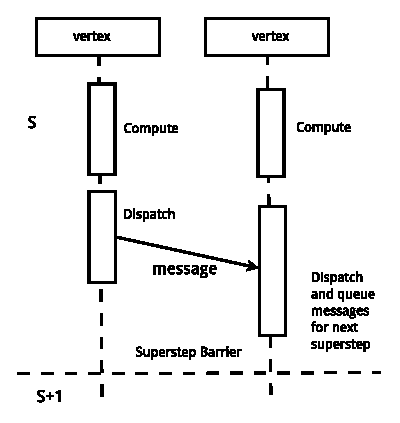
\includegraphics[width=0.8\textwidth,angle=0]{figure/sequentialbsp_new.eps}
\end{minipage}
    \caption{\textbf{Sequential BSP model}}
    \label{figure:sequentialbsp}
\end{figure}



\section{System Design}

In order to improvement the vertex-centric model, we overlap the compute and dispatch procedure and introduce our new BSP model. Then we analysis the data behavior based the new BSP model with actors during processing. And Finally, based on our investigation, we describe the data arrangement of the GPSA.

\subsection{New BSP model with Actors}
 
Actors should reponse to messages, so does the computation procedure. Actors generate messages, so does the dispatch procedure. In New BSP model, we dilute the concept of vertex-cenric because of the inefficiency mentioned above. Therefore, there are two different roles in our computation model, dispatcher and computer , As shown in Figure \ref{figure:computemodel}. The main responsibility of dispatch actor is sending messages to compute actors. While the compute actor is responsible for computing received messages. From the perspective of actors, vertices and edges are the material of messages. When all dispatchers and computers finished their work, the model will start the next iteration with superstep increment by 1. In the New BSP model, not matter dispatchers or computers, they are the basic execute unit and all the message passing among vertices via actors. Instead of storing the messages or combining messages for the next superstep like the raditional BSP model, the compute actors consume the messages immediately once they receive the messages. By that way, there is a little different from the traditional BSP model. In traditional way, there always have a superstep 0 to send messages and does not caculate at all. However, in the New BSP model, it start caculate once the processing started. When an actor need to send a message, it does not have to wait for the computation of the current iteration to finish and send the messages directly because the computation for the current iteration has already been finished in the last iteration. \newline

\begin{figure}[htbp]

\begin{minipage}[]{0.5\textwidth}
	\centering
     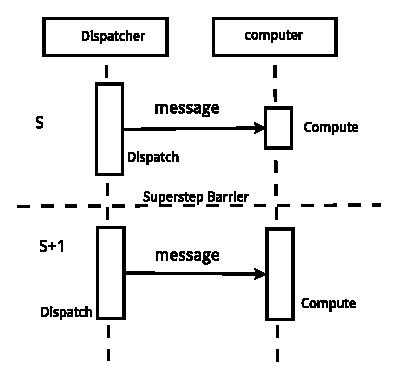
\includegraphics[width=0.8\textwidth,angle=0]{figure/computemodel.eps}
\end{minipage}
    \caption{\textbf{compute model with actors}}
    \label{figure:computemodel}
\end{figure}




\subsection{Data Behavior}

First, we assume that each actor is mapped to a vertex. Though there is no superstep conceptually, the most common thing is message. The message-passing between vertices is transformed into communication between actors. For a vertex or actor $V$, it does not care in which order or how messages coming. It only concerns message values and what to with these values. A message usually consists of destination and value. To process a message, the first thing is that find the value of the destination vertex $V$, then invoke the user defined $compute$ method. Actors responses to messages, However, as messages coming randomly, this will cause random access problem which other single machine spare no effort to avoid. Once actors receive a message, the value of a specified vertex should be available not matter it is in memory or on the hardware. 
Second, we observe that based on the New BSP model, there is a need to store two copy of values, one copy is for dispatching and the another is for updating. For the dispatcher, the updated value need to inform its neighbour vertex, thus dispatch procedure. And For compute actor, the new value of compute should be updated for next superstep, thus compute procedure. Therefore, to implement actor based graph processing system, a fast data access technology is essential. 

\subsection{Memory Mapping}

As mentioned above, the data behavior of actor is quick random access which is a issue in other approaches. Our purpose is a new computation model, so how to slove this problem is not in our concern, but we still provided a solution. In fact, memory mapping is one of the basic function of modern operation system. The primary benefit of memory mapping is mechanism that maps a portion of a file, or an entire file on disk to a range of addresses within an application's addres space. The application can then access files on disk in the same way it access dynamic memory.\newline

In a 32-bit operating systems, memory-mapped files is usually used for high speed disk access. However, due to the limited address space of the 32-bit operating system, memory-mapped file is less likely used for massive virtual memory or for large files. While in a 64-bit operating system, memory-mapped files can map TB or even PB of memory into a process’s address space. Now that the JVM is 64-bit and could runs on 64-bit operation system, the JAVA developer doesn’t need to consider the disk and the memory as being separate things and could combine them with memory-mapped files via the MappedByteBuffer class. With memory-mapping, the process does not need to bother itself about whether the memory is in RAM or on the disk. \newline

\subsection{Data Arrangement}

In order to slove the random access issue, we take advantage of the memory mapping. Values of vertices are stored in a single file in order, i.e. the value offset of vertex $V$ is $|V|*sizeof(Val)$. Through memory mapping, we can access these data randomly as like we are operating an normal big array. Furthermore, we store the value in two columns to solve the problem we mentioned in Section Data Behavior and will be detailed in next section. \newline
For dispatchers, there are more data to access, i.e. the edges. For the sake of saving memory and improve IO performance, we store store graph in Compressed Sparse Row (CSR) format. As the CSR do not provide any mutability. We sperate the vertex value from the graph.  However, the CSR format stores vertices and edges in separate arrays, with the indices into these arrays corresponding to the identifier for the vertex or edge, respectively. The edge array is sorted by the source of each edge, but contains only the targets for the edges. The vertex array stores offsets into the edge array, providing the offset of the first edge outgoing from each vertex. Iteration over the out-edges for the ith vertex in the graph is achieved by visiting $edge_array[vertex_array[i]]$, $edge_ array[vertex_array[i]+1]$, ..., $edge_ array[vertex_array[i+1]]$. For example, in figure \ref{figure:csrexample}, vertex $0$ has two out-edges pointing to vertex  $2$ and vertex $3$, and the $-1$ indicates that the edges of current vertex is over. In 

In fact, with the New BSP model, the vertex-centric is diluted into actor-centric. Actor does not care vertex. Actor only cares vaue and messages. So it is able to process original edge list without preprocess. However, with preprocess, arrange graph data in CSR format could have more flexiability, for example, advanced message combine which will combine some messages to same compute actor into one messages. Especially, in some application, the outdegree of the vertex matters, with CSR data format, we will be able to store this information in file and save a lot of enery to caculate it, as shown in figure \ref{figure:csrexample}.


\begin{figure}[htbp]

 \begin{minipage}[]{0.5\textwidth}
 \centering
     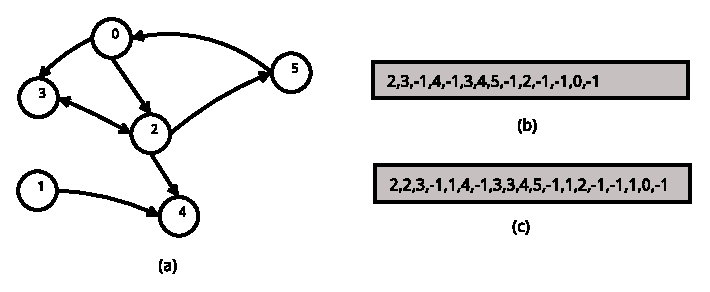
\includegraphics[width=0.8\textwidth,angle=0,scale=1.2]{figure/csrdataformat.eps}
\end{minipage}
    \caption{\textbf{CSR example}  }
	\textit{(a) a example graph (b) a csrfile content without vertex degree (c) csrfile content with vertex degree}
    \label{figure:csrexample} 
\end{figure}

\subsection{Message Dispatching}
A message consists of message value and the destination vertex id. In some application, the message value is the update value of a vertex, sometimes it related to both the value and the outdegree in other applications like PageRank. Therefore, we ask the developer to implement the details of how to generate a message value according to the vertex value, outdegree and even the edge weight. If a vertex value has been updated in the last iteration, once the dispatcher worker start to process the updated vertex, it will invoke the user supply method to generate the message value. Then the dispatcher pack the value with the integer id together and locate the compute worker who will process this message according to the destination id. In fact, there is a great chance that the different adjacent out-edges of a vertex will locate the same compute worker. If the message value has nothing to do with the outdegree or the edge weight, it usually has the same value actually. Packing multi-id with a message value will reduce the number of the message greatly. Otherwise, if the vertex value did not updated, the dispatcher will skip it.

To delivery a message to a specific compute actor, there are several strategies. The most easiest way is a average assignment by mod according the vertex id. In this way, every single compute actor will not have conflict with others when updating. However, it may cause the unblance worklod among 

\subsection{Updating}

We store values in two column, actually, two copies of values of two different vlaues. One copy is the result of last superstep, while the other is the result of the superstep before the last superstep. And values of last superstep will be used to dispatching, and the other will be overwrite. In fact, all the values stored in the file is in a sequential way, for the perspective of vertex id, it looks like two columns, as shown in figure \ref{figure:vu}. \newline
For a compute actor, two mainly problems may occur. First, the value in the mapped file is stored in two column way for each vertex. One column is used for message sending, the other is used for updating. After a iteration,  two columns of values will become different. So if the compute worker fetch value directly, it will get the wrong data because the validate value is stored in the message sending column actually. So there is a need for the compute worker to figure out the first message of a vertex and fetch value from the message sending column then write it into the updating column. \newline
Second, as mentioned in the last section, if a vertex value is not updated, the dispatcher will skip it. Messages come randomly, it is hard to identify whether a value is updated or not. Though the compute worker knows the updating happened, it has no idead of what to do with it. In order to share the update information with the dispatcher, we set the highest bit of the value to 1, which is negative. At first, all the value will be set. During the computation, if a value has been updated, the highest bit will be reset to 0 and write the update. Otherwise, if a message is the first message of the vertex, the negative value will be written. After a dispatcher finish the dispatching procedure of a vertex, the dispatcher will disable the value of the current vertex, which means to set the highest bit of the value to 1. For example, in figure \ref{figure:vu}, values of two columns are exactly the same according the initialize function supplied by the user. And the initial value are all setted at highest bit. In superstep 0, dispatchers read from the first column, left side, and compute actors update into the second column , right side. If a value is updated, its highest bit is set to 0, like the 0x00000001 and 0x00000002. In superstep 1, the dispatchers read from the second column and compute worker update the first column. And in each superstep, the dispatcher disabled the value by setting the highest bit to 1. When there are no more messages, the computation is over.

\begin{figure}[!htbp] 
\centering
 \begin{minipage}[]{1.2\textwidth}
     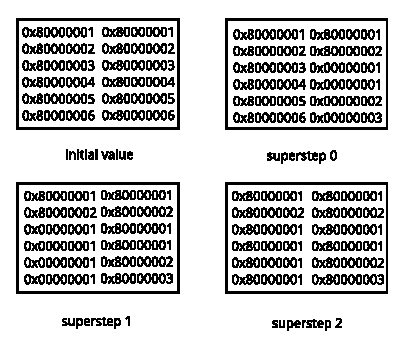
\includegraphics[width=0.4\textwidth,angle=0]{figure/Valueupdating.eps}
\end{minipage}
    \caption{\textbf{Value updating}}
    \label{figure:vu}
\end{figure}


\subsection{Cheap Fault Tolerant}
Fault tolerant is important to guarantee the reliability of the system, especially for the high-performance demands. For a graph processing system, a fault-tolerant system must keep track of the whole state of the graph. In GPSA, the graph data is stored in unmutable format, so we can achieve fault tolerant purpose easily. All values are stored  in two-column format. In a superstep, there is always a column is unmutable, which ensure that there is always a copy of right result of the last iteration stored. If the system crash in the current iteration, we can recover the system from the latest successfully finished iteration.

Furthermore, we take advantage of actors to implement GPSA. We arrange our actors in a manager-worker hierarchy. At the bottom is the dispatcher worker actors and the main computational unit worker. While upon the worker actors is the manager actors who is responsible for global coordinating and monitoring . Because the main purpose of the actor model is to break down the large task into small tasks. During the processing, if an actor throws an exception, for the performance reason, the manager actor will handle the exception. If the manager actor also have no idea what to do with the exception, then this exception will report to the supervisor manager actor. \newline



\section{Implementation}

We implemented GPSA in Java. The actor library is Kilim and the IO is mainly take advantage of memory mapping. And all the data file is stored on disk with binary format as mentioned above.

\subsection{Overview}

Similar to the GraphChi, we also assume that the vertices are labeled from $0$ to $|V|$ but unlike Graphchi, we uses the compressed sparse row storage format to store the graph in a binary mapped file . And an entry of a vertex is separated by a separator symbol. During the processing, each dispatcher worker will read the mapped file to get the out edges to send messages. In fact, there are different ways to read mapped files to manager the load balance among workers. For example, for the sake of convenience, the vertices can be read by the dispatch actors with a simple mod algorithm. For efficient, assigning these vertices to the dispatcher worker by the average edges to ensure that every dispatcher worker send exactly the same messages. At the same time, the value of the vertex is stored in another mapped file. And each value of the vertex are stored in a memory mapped file in ascending order by its label. In this way, we can access the data in a sequential way like a normal array. For example, for a vertex whose id is k, the start index of its value stored in the mapped file could be figure out by the equation $index = id * sizeof(value)*factor$. 





\begin{thebibliography}{00}
\setlength{\itemsep}{0pt}
    
	\bibitem{http}LMAX Disruptor High Performance Inter-Thread Messaging Library. http://lmax-exchange.github.io/disruptor/

     \bibitem{Kyrola}Kyrola A, Blelloch G, Guestrin C. GraphChi: Large-scale graph computation on just a PC[C]//Proceedings of the 10th USENIX Symposium on Operating Systems Design and Implementation (OSDI). 2012: 31-46.
    \bibitem{xstream}Roy A, Mihailovic I, Zwaenepoel W. X-Stream: edge-centric graph processing using streaming partitions[C]//Proceedings of the Twenty-Fourth ACM Symposium on Operating Systems Principles. ACM, 2013: 472-488.
    
    \bibitem{Cheng}R. Cheng, J. Hong, A. Kyrola, Y. Miao, X. Weng, M. Wu,F. Yang, L. Zhou, F. Zhao, and E. Chen. Kineograph: Taking the Pulse of a Fast-Changing and Connected World. In Proceedings of the 7th ACM european conference on Computer Systems (EuroSys), pages 85–98, Bern, Switzerland, 2012.
    
    \bibitem{Dean}Jeffrey Dean and Sanjay Ghemawat, MapReduce:Simplified Data Processing on Large Clusters. in Proc.6th USENIX Symp. on Operating Syst. Design and Impl.,2004, 137–150.
    \bibitem{Han}Han W S, Lee S, Park K, et al. TurboGraph: a fast parallel graph engine handling billion-scale graphs in a single PC[C]//Proceedings of the 19th ACM SIGKDD international conference on Knowledge discovery and data mining. ACM, 2013: 77-85.
    
    \bibitem{Hong}S. Hong, H. Chafi, E. Sedlar, and K. Olukotun.Green-Marl: A DSL for Easy and Efficient  Graph Analysis.In ASPLOS, 2012.
    \bibitem{Hong}Hong S, Salihoglu S, Widom J, et al. Tech Report: Compiling Green-Marl into GPS[J]. 2012.
    
    \bibitem{J E}Gonzalez J E, Low Y, Gu H, et al. Powergraph: Distributed graph-parallel computation on natural graphs[C]//Proceedings of the 10th USENIX Symposium on Operating Systems Design and Implementation (OSDI). 2012: 17-30.
    
    \bibitem{Kang}U. Kang, C. E. Tsourakakis, and C. Faloutsos. Pegasus: A peta-scale graph mining system - implementation and observations. In ICDM,pages 229–238, 2009.
   \bibitem{Kang}U. Kang, H. Tong, J. Sun, C.-Y. Lin, and C. Faloutsos. Gbase: a scalable and general graph management system. In KDD, pages 1091–1099, 2011.
	\bibitem{Kang}U. Kang, H. Tong, J. Sun, C.-Y. Lin, and C. Faloutsos. gbase: an efficient analysis platform for large graphs. VLDB J., 21(5):637–650,2012.
    
    \bibitem{Lumsdaine}A. Lumsdaine, D. Gregor, B. Hendrickson, and J. Berry. Challenges in parallel graph processing. Parallel Processing Letters, 17(1):5–20, 2007.
    
    \bibitem{M}Karp R M. A survey of parallel algorithms for shared-memory machines[J]. 1988.
    \bibitem{Malewicz}G. Malewicz, M. H. Austern, A. J. Bik, J. C. Dehnert,I. Horn, N. Leiser, and G. Czajkowski. Pregel: a system for large-scale graph processing. In SIGMOD’10, pages 135–146, New York, NY, USA, 2010. ACM.
   \bibitem{actoronjvm} Karmani R K, Shali A, Agha G. Actor frameworks for the JVM platform: a comparative analysis[C]//Proceedings of the 7th International Conference on Principles and Practice of Programming in Java. ACM, 2009: 11-20.
\bibitem{Pearce}R. Pearce, M. Gokhale, and N. Amato. Multithreaded 2011.Asynchronous Graph Traversal for In-Memory and Semi-External Memory. In SuperComputing, 2010.

    \bibitem{Pujol}J. M. Pujol, V. Erramilli, G. Siganos, X. Yang, N. Laoutaris, P. Chhabra, and P. Rodriguez. The Little Engine(s) That Could: Scaling Online Social Networks. IEEE/ACM Transactions on Networking, 20(4):1162–1175, 2012.
    \bibitem{S}Srinivasan S, Mycroft A. Kilim: Isolation-typed actors for java[M]//ECOOP 2008–Object-Oriented Programming. Springer Berlin Heidelberg, 2008: 104-128.
\bibitem{S}Srinivasan S. Kilim: A server framework with lightweight actors, isolation types and zero-copy messaging[J]. University of Cambridge, Computer Laboratory, Technical Report, 2010 (UCAM-CL-TR-769).
\bibitem{S}Srinivasan S. A thread of one’s own[C]//Workshop on New Horizons in Compilers. 2006, 4.
    \bibitem{S}Salihoglu S, Widom J. Gps: A graph processing system[C]//Proceedings of the 25th International Conference on Scientific and Statistical Database Management. ACM, 2013: 22.
	\bibitem{Shun}Shun J, Blelloch G E. Ligra: a lightweight graph processing framework for shared memory[C]//Proceedings of the 18th ACM SIGPLAN symposium on Principles and practice of parallel programming. ACM, 2013: 135-146.

\bibitem{V}Prabhakaran V, Wu M, Weng X, et al. Managing large graphs on multi-cores with graph awareness[C]//USENIX ATC. 2012, 12.
\bibitem{Valiant}Leslie G. Valiant, A Bridging Model for Parallel Computation. Comm. ACM 33(8), 1990, 103–111.

\bibitem{Y}Low Y, Gonzalez J, Kyrola A, et al. Graphlab: A new framework for parallel machine learning. arXiv preprint[J]. arXiv preprint arXiv:1006.4990, 2010.

\bibitem{Z}Khayyat Z, Awara K, Alonazi A, et al. Mizan: a system for dynamic load balancing in large-scale graph processing[C]//Proceedings of the 8th ACM European Conference on Computer Systems. ACM, 2013: 169-182.

\end{thebibliography}

\end{document}